\chapter{Réalisation}\label{realisation}


\section{Capture d'image}\label{realisation.capture}
\subsection{Emplacement de la caméra}
La photo présentée en figure \ref{fig:cam_parking_annotation} est une image satellite du site de Cheseaux de la HEIG-VD. C'est ici qu'un parking sera filmé à l'aide d'une caméra.

\begin{figure}[H]
    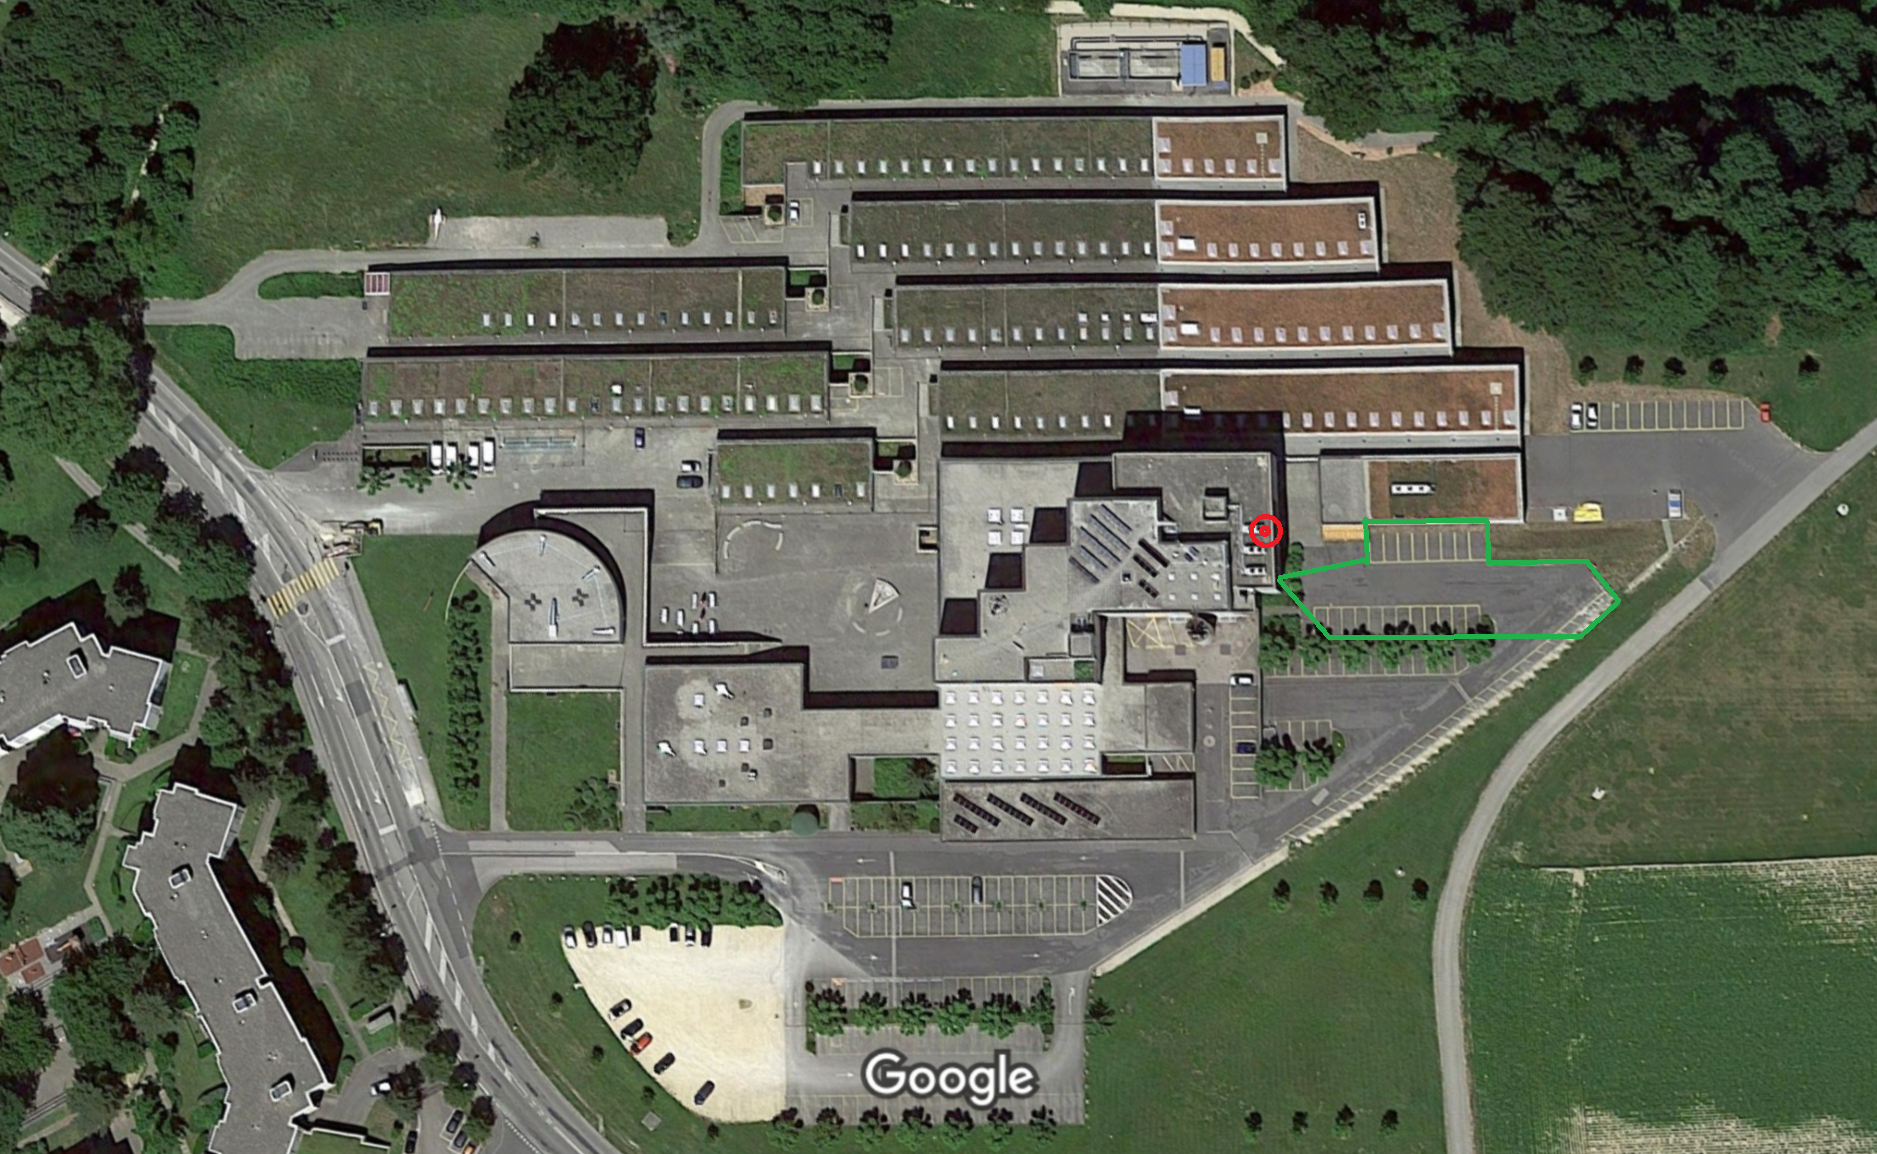
\includegraphics[width=130mm]{img/conception/cam_parking_location.png}
    \label{fig:cam_parking_annotation}
    \centering
    \captionsource{Emplacement de la caméra (en rouge) et du parking filmé (en vert)}{map:heig-vd}
\end{figure} 

Y est désigné par un cercle rouge l'emplacement de la caméra. Elle se situe sur la terrasse du bâtiment est, accessible au niveau K. Elle est orientée vers le parking désigné en vert. 

\subsection{Requêtes et protocole}

\subsection{Monitoring}

\section{Traitement des images}
\subsection{Downsampling}
\subsection{Détection de bord}
\subsection{Evaluation des différentes méthodes et choix}

\section{Annotations des images}

\section{Définition du réseau de neurone}

\section{Entrainement du modèle}




\todo{schéma dialogue caméra + edge detection déjà fait}

